% !TEX root = _individual/trtBackground.tex

%%%%%%%%%%%%%%%%%%%%%%%%%%%%%%%%%%%%%%%%%%%%%%%%%%%%%%%%%%%%%%%%%%%%%%%%%%%%%%%%
\chapter{Background to Thermal Radiative Transfer}\label{chap:trtBackground}

In order to elucidate the derivation and application of the anisotropic
diffusion approximation, it is necessary to delve deeper into the physical
process that is subject to the approximation. As discussed in the introduction,
thermal radiative transfer is the physical process of energy transfer via
high-energy photons in hot materials. Because the TRT equations and
approximations have been probed and reviewed in countless other works
\cite{Mih1984,Pom1973,Cas2004,Wol2008}, our aim is a concise explanation of the
physics relevant to the anisotropic diffusion approximation and its immediate
application, rather than a thorough overview of the extensive field of radiation
hydrodynamics. We also review the derivation of competing solution methods and
discuss their advantages and shortcomings.

%%%%%%%%%%%%%%%%%%%%%%%%%%%%%%%%%%%%%%%%%%%%%%%%%%%%%%%%%%%%%%%%%%%%%%%%%%%%%%%%
\section{Equations of transfer}\label{sec:trtEquations}
Thermal radiative transfer describes how high-energy photons move energy about
in a very hot material, such as the interior of a star or the target of a laser
fusion experiment. The equations that model TRT are time-dependent, contain
strong nonlinearities, and reside in a large phase space.
A full representation of the physics in
the high-energy-density regime often includes the consideration of moving
relativistic materials, different electron and ion temperatures, photon
scattering, and thermal conduction in the material \cite{Mih1984}. However,
much theoretical work in the field neglects these complex phenomena by
\begin{itemize}
  \item working in a fixed medium, disregarding material advection;
  \item assuming local thermodynamic equilibrium (LTE), which uses a single
    material temperature;
  \item neglecting photon scattering, which tends to be comparatively small for
    very hot materials; and
  \item neglecting thermal conduction, since energy transfer is dominated by
    radiation in the temperature regimes we consider.
\end{itemize}

A further simplification often used for methods development is the ``gray''
approximation to the frequency dependence. Analogous to the one-group
approximation for neutron transport, the full transport equation is integrated
over all frequencies, and the opacities are averaged with some \emph{a priori}
weighting function, typically the Rosseland mean \cite{Lar1983a}.

For the purposes of discussion and the later AD derivation, we consider a
general, 3-D universe, where the spatial coordinates are
\begin{equation*}
  \vec{x}
  = x \vec{i} + y \vec{j} + z \vec{k}\,,
\end{equation*}
and the angular coordinates are the unit vector
\begin{equation*}
  \vec{\Omega}
  = \mu \vec{i}
  + \sqrt{1-\mu^2} \cos \theta \vec{j}
  + \sqrt{1-\mu^2} \sin \theta \vec{k} \,.
\end{equation*}
These angular coordinates reside in the domain $-1 \le \mu \le 1$, $0 \le \theta
< \pi$; we use $\vec{\Omega}\in4\pi$ as a frequent shorthand denoting the entire
unit sphere. See \cite{Lar2007,Pri2010} for a more complete discussion of the
spatial and angular coordinate systems.

After the simplifications described above, the thermal radiative transfer
process in the interior of a problem (away from the initial time and
from boundaries) can be described by
\begin{subequations} \label{eqs:explanTRT}
the radiative transfer equation,
\begin{equation} \label{eq:explanTransport}
  \frac{1}{c} \pder{I}{t}
  + \vec{\Omega} \vd \del I +
 \sigma I
  = \frac{\sigma a c T^4}{4\pi} 
  + \frac{c q_r}{4\pi} \,,
\end{equation}
and the material energy balance equation,
\begin{equation} \label{eq:explanMaterial}
  c_v \pder{T}{t} = \sigma \int_{4\pi}  I \ud \Omega - \sigma a c T^4 \,.
\end{equation}
\end{subequations}

The notation and omitted parameters in Eqs.~\eqref{eqs:explanTRT} are:
\begin{alignat*}{2}
  I &= I(\vec{x}, \vec{\Omega}, t) &&= \text{the angular
  radiation intensity,}
  \\
  T &= T(\vec{x}, t) &&= \text{the material temperature,}
  \\
  \sigma &= \sigma(\vec{x}, T) &&= \text{the absorption opacity,} 
  \\
  q_r &= q_r(\vec{x}, t) &&= \text{an extraneous isotropic radiation energy source,}
  \\
  c_v &= c_v(\vec{x}, T) &&= \text{the specific heat capacity of a material,}
  \\
  a& &&= \text{the radiation constant, and}
  \\
  c& &&= \text{the speed of light.}
\end{alignat*}
The intensity $I$ and the temperature $T$ are the primary unknowns: they
describe the state of energy in the radiation and in the material.
Each of the terms that depends on $T$ implicitly depends on the time $t$. The
explicit dependence of $c_v$ and $\sigma$ on $\vec{x}$ accounts for different
materials in different parts of the problem.

Equation~\eqref{eq:explanTransport} is a transport equation for $I$. The first
two terms describe how photons ``stream'' in time and space: if the $\sigma$
and source terms were zero, Eq.~\eqref{eq:explanTransport} would reduce to a
wave equation with a wave speed of $c$. However, because the photons are moving
through a material, there is a chance they will collide with the material,
hence the \emph{collision} term $\sigma I$. The first term on the right-hand
side represents particles emitted via the isotropic temperature-dependent
process of black body emission. The additional term $q_r$ is an extraneous
isotropic radiation source that emits with an energy density (energy per
volume per time) of $q_r$.

The material equation~\eqref{eq:explanMaterial} describes an energy balance in
the material. On the left-hand side is the time rate of change in the material
energy density, which is a function of the material's temperature and specific
heat capacity $c_v$:
\begin{equation} \label{eq:matEnergyDens}
  U_m(T) = \int_{0}^{T} c_v(T') \ud T' \,.
\end{equation}
The first term on the right hand side exactly mirrors the collision term in the
radiation equation: it is a ``gain'' term corresponding to photons that
collided with (were absorbed by) the material. The second term describes when
energy is lost from the material and emitted as radiation: black body emission.

In order to conserve energy in a simulation, strict attention must be paid to
$U_m$ and $\phi$, which are the true quantities of energy in
the material and radiation. If the loss, gain, and rate of change terms are not
properly treated, energy will not be conserved.

The physical properties $\sigma$ and $c_v$ are often approximated by simplistic
models in the methods development sphere. The heat capacity $c_v$ of an ideal
gas is a constant, giving the material energy $U_m$ a linear proportionality to
the material temperature $T$. A much-used model \cite{Mou2006,Wol2008} of the
gray opacity is $\sigma \propto \propto T^{-3}$.
Our numerical test problems will use both of these idealized representations of
the physical constants.

The nonlinear coupling between Eqs.~\eqref{eq:explanTransport}
and~\eqref{eq:explanMaterial} via $T^4$ emission and $T^{-3}$ absorption make
the TRT equations extremely ``stiff'' \cite{Kno2003} and therefore even more
difficult to solve than the standard linear transport equation. In this work,
we will not attempt to provide any new solutions to treat the nonlinearities,
but we will formulate our time-dependent anisotropic diffusion approximations to
be compatible with multiple solution techniques.

\subsection{The radiation intensity}

In radiative transfer, the intensity $I$ is the energy-weighted radiation path
length density, similar to the angular flux $\psi$ in reactor physics:
\begin{align*}
  I(\vec{x},\vec{\Omega},\nu, t) &= c h\nu N(\vec{x},\vec{\Omega},\nu, t)\,,
  \\
  \intertext{where $h\nu$ is the photon energy and $N$ is the photon density,}
  N(\vec{x},\vec{\Omega}, \nu, t) \ud V \ud \Omega
  &= \topbox{the number of photons inside the differential volume $\ud V$
  about $\vec{x}$, traveling in the directions $\Omega$ about
  $\vec{\Omega}$, inside the frequencies $\ud \nu$ about $\nu$, at time $t$.}
\end{align*}
Integrating over all energy gives the gray intensity,
\begin{equation*}
  I(\vec{x},\vec{\Omega}, t)
  = c \int_0^\infty h\nu N(\vec{x},\vec{\Omega},\nu, t) \ud\nu \,.
\end{equation*}

Additionally, integrating over all angles (i.e.~taking the zeroth angular
moment) yields the ``scalar intensity''
\begin{align} \label{eq:intensityZeroth}
  \phi(\vec{x},t) &\equiv \int_{4\pi} I(\vec{x},\vec{\Omega}, t) \ud \Omega
  \\
  &= c \int_{4\pi} \int_0^\infty h\nu N(\vec{x},\vec{\Omega},\nu, t) \ud\nu
   \ud \Omega
\\ \intertext{which is directly proportional to the radiation energy density:}
\nonumber
\frac{1}{c} \phi(\vec{x},t) \ud V
&= \topbox{the amount of energy in the radiation field inside the differential
  volume $\ud V$ about $\vec{x}$, at time $t$.}
\end{align}
For our work, it is usually more convenient to refer to $\phi$ than to the
radiation energy density (compare, for example, \cite{Den2007} to
\cite{Kno1999a}). In fact, since in our computational experiments we use the
scaled system of variables $c=a=1$, our later results can use ``scalar
intensity'' and ``radiation energy density'' interchangeably.

The first angular moment of the intensity also has physical significance. The
radiation flux is defined as
\begin{equation} \label{eq:intensityFirst}
  \vec{F}(\vec{x},t) \equiv \int_{4\pi} \vec{\Omega}
  I(\vec{x},\vec{\Omega}, t) \ud \Omega \,.
\end{equation}
Analogous to the ``neutron current'' $\vec{J}$ in reactor physics, the
radiation flux is the net rate of energy flowing through a point.

At any particular point in space and time, the radiation intensity $I$ is
generally a complicated function of angle. For example, at the edge of a
radiation shock wave, the distribution is highly peaked in the directions
pointed away from the hot region, because that is the source of the photons. In
other parts of the problem where the system is closer to an equilibrium state,
the intensity is nearly isotropic: that is, the intensity is almost a uniform
function in angle.

\subsection{Initial and boundary conditions}
The problem of interest lies in a convex region $V$ that has an exterior surface
$\partial V$: the transport equation Eq.~\eqref{eq:explanTransport} is valid
for $\vec{x} \in V$, and boundary conditions are needed to describe the
intensity $I$ for incoming angles, $\vec{\Omega}\vd \vec{n} < 0$ for $\vec{x}\in
\partial V$. Here, $\vec{n}$ is the outward surface normal vector at a point on
the boundary.

The transport equation and material are time-dependent, and accordingly they
need initial conditions. In the context of the work in this thesis, the simplest
time range to use is $0 \le t \le \Delta_t$, a single time step. The value of
the material and radiation temperature at $t=0$ are either a user-specified
initial condition or the latest solution with the clock reset to zero.

%%%%%%%%%%%%%%%%%%%%%%%%%%%%%%%%%%%%%%%%%%%%%%%%%%%%%%%%%%%%%%%%%%%%%%%%%%%%%%%%
\section{Radiation transport approximations}\label{sec:trtApproxMethods}

The large phase space and nonlinearity of Eqs.~\eqref{eqs:explanTRT} makes a
direct solution intractable except for the simplest of problems
\cite{Su1997,Mos2006}. A more complete overview of the approximations is given
in \cite{Bru2002,Ols2000,Wol2008}.

All of the approximations trade speed for accuracy. The fewer unknowns a method
has, the easier it is to solve.

The treatment of the angular distribution of $I$ is the
primary difference between the radiation transport approximations. The
anisotropic diffusion methods we derive later in this thesis use an
approximation entirely different from existing methods.

%%%%%%%%%%%%%%%%%%%%%%%%%%%%%%%%%%%%%%%%
\subsection{Implicit Monte Carlo}

\begin{itemize}
  \item linearized $\sigma$, $B$ (semi-implicit)
  \item typical MC is exact, whereas nonlinearities in IMC incur spatial
    discretization and $O(\Delta_t)$ linearization error
  \item expensive: storage of particle census
\end{itemize}

%%%%%%%%%%%%%%%%%%%%%%%%%%%%%%%%%%%%%%%%
\subsection{Discrete ordinates}

Additional spatial, angular, and temporal discretization errors

%%%%%%%%%%%%%%%%%%%%%%%%%%%%%%%%%%%%%%%%
\subsection{Spherical harmonics}
\cite{Ols2000,McC2008a}

VEF, \Pone

%%%%%%%%%%%%%%%%%%%%%%%%%%%%%%%%%%%%%%%%
\subsection{Diffusion}\label{sec:diffusion}

Angular approximations

%%%%%%%%%%%%%%%%%%%%%%%%%%%%%%%%%%%%%%%%
\subsection{Flux-limited diffusion}\label{sec:fldBackground}

The radiation intensity satisfies the mathematical identity $\norm{F} \le \phi$,
essentially limiting the leakage of radiation at a point to the radiation
energy at that point. The identity can be proven using the triangle inequality:
\begin{align*}
  \norm{\vec{F}} &= \norm{ \int_{4\pi} \vec{\Omega} I \ud \Omega}
  \\&\le \int_{4\pi} \norm{\vec{\Omega}} \abs{I} \ud \Omega 
  \\
  &\le \int_{4\pi} [1] I \ud\Omega
  \\
  \norm{\vec{F}} &\le \phi\,.
  \\ 
  \intertext{Substituting Fick's law for $\vec{F}$ gives a condition that the
  diffusion coefficient should ideally satisfy in the presence of large
  gradients:}
  \norm{- D \grad \phi} &\le \phi
  \\
  D & \le \frac{\phi}{\norm{\grad \phi}} \,.
\end{align*}

\subsubsection{Flux limiters}

\subsubsection{Flux limiter discretization}
\cite{Ols2007}

%%%%%%%%%%%%%%%%%%%%%%%%%%%%%%%%%%%%%%%%%%%%%%%%%%%%%%%%%%%%%%%%%%%%%%%%%%%%%%%%
\section{Semi-implicit linearization}

To solve the TRT equations with deterministic methods, we use a semi-implicit time
discretization scheme \cite{Kno1999a,Kno2001,Low2004} where some important
unknowns are treated implicitly in
time, and other unknowns are treated explicitly. 
Equations~\eqref{eqs:explanTRT} can be formulated as a time-dependent linear
transport equation over a time step $t^n < t < t^{n+1}$.

For the semi-implicit discretization, it is more convenient to write
Eqs.~\eqref{eqs:explanTRT} in a slightly altered form:
\begin{subequations} \label{eqs:semiTRT}
\begin{equation} \label{eq:semiTransport}
  \frac{1}{c} \pder{I}{t}
  + \vec{\Omega} \vd \del I +
 \sigma I
 = \frac{\sigma c U_r}{4\pi} 
  + \frac{c q_r}{4\pi} \,,
\end{equation}
and the material energy balance equation,
\begin{equation} \label{eq:semiMaterial}
  \pder{U_m}{t} = \sigma \int_{4\pi}  I \ud \Omega - \sigma c U_r \,.
\end{equation}
\end{subequations}
Here, we have defined the ``equilibrium radiation energy density'' of a
material as a scaled integral of the Planckian emission function:
\begin{equation} \label{eq:radEnergyDens}
  U_r(T) \equiv aT^4
  = \frac{1}{c} \int_{4\pi} \int_{0}^{\infty} B(\nu, T) \ud\nu \ud\Omega \,.
\end{equation}
Its physical relevance is that, when the radiation field and material reach
an equilibrium, $I=B$, and the radiation energy density $\phi/c$ is equal to
$U_r$.  The quantity $U_r$ is \emph{not} equal to the energy density stored in
the material, $U_m$.

\subsection{Linearizing the material energy equation}

First, we define a parameter $\beta$ as a function of
Eqs.~\eqref{eq:matEnergyDens} and~\eqref{eq:radEnergyDens}:
\begin{equation} \label{eq:beta}
  \beta(\vec{x}, T) \equiv \pder{U_r}{U_m} 
  = \pder{U_r}{T} \Bigg/ \pder{U_m}{T}
  = \frac{4 a T^3}{c_v(\vec{x}, T)} \,.
\end{equation}
The chain rule allows the left hand side of Eq.~\eqref{eq:semiMaterial} to be
expressed without approximation in terms of the equilibrium radiation energy
density $U_r$:
\begin{equation*}
  \pder{U_m}{t} = \pder{U_m}{U_r} \pder{U_r}{t} = \frac{1}{\beta(T)}
  \pder{U_r}{t} = \sigma \int_{4\pi}  I \ud \Omega - \sigma c U_r \,.
\end{equation*}
The first approximation is to ``freeze'' the parameter $\beta$ at the beginning-of-time-step temperature $T^n$:
\begin{equation}\label{eq:frozenBeta}
  \frac{1}{\beta^n}
  \pder{U_r}{t} \approx \sigma \int_{4\pi}  I \ud \Omega - \sigma c U_r \,.
\end{equation}
The process of freezing $\beta$ is equivalent to approximating the
Planckian emission term with a Taylor series \cite{Kno2007}.

Because the approximation to $\beta$ is an approximation to the rate of change
in material energy, this equation no longer conserves the system's total
energy. To enforce conservation of energy over a time step, we must set the
material energy change over a time step to the time-integrated approximation:
\begin{align}
  \nonumber
  \int_{t^n}^{t^{n+1}}  \pder{U_m}{t}\ud t &= \frac{1}{\beta^n}
  \int_{t^n}^{t^{n+1}} \pder{U_r}{t}\ud t
  \\
  \nonumber
  U_m^{n+1} - U_m^n &= \frac{1}{\beta^n} \left[ U_r^{n+1} - U_r^n \right]
  \\
  \label{eq:matenConservationUpdate}
  U_m^{n+1} &=  U_m^n + \frac{U_r^{n+1} - U_r^n}{\beta^n}\,.
\end{align}
%Thus, the expression of $\tpder{U_m}{t}$ in terms of $\tpder{U_r}{t}$

The next approximation is to explicitly freeze the opacity $\sigma$ in
Eq.~\eqref{eq:frozenBeta}:
\begin{equation*}
  \frac{1}{\beta^n}
  \pder{U_r}{t} \approx \sigma^n \int_{4\pi}  I \ud \Omega - \sigma^n c U_r \,.
\end{equation*}
Now we can time-average the material equation to express it in terms of two
simple time-average unknowns. Operating by
$\frac{1}{\Delta_t^n}\int_{t_n}^{t^{n+1}} (\cdot) \ud t$,
\begin{equation*}
  \frac{1}{\beta^n}
  \frac{U_r^{n+1} - U_r^n}{\Delta_t^n} = \sigma^n \int_{4\pi} \left[
  \frac{1}{\Delta_t^n}\int_{t_n}^{t^{n+1}} I\ud t
  \right] \ud \Omega - \sigma^n c \left[
  \frac{1}{\Delta_t^n}\int_{t_n}^{t^{n+1}} U_r \ud t \right]\,.
\end{equation*}
Next, we apply the implicit Euler approximation to $U_r(\vec{x}, \vec{\Omega},
t)$ and $I(\vec{x}, \vec{\Omega}, t)$ by setting their time-averaged values to
the values at $t^{n+1}$:
\begin{equation} \label{eq:semiImplicitMaterial}
  \frac{1}{\beta^n(\vec{x})}
  \frac{U_r^{n+1}(\vec{x}) - U_r^n(\vec{x})}{\Delta_t^n}
  = \sigma^n(\vec{x}) \int_{4\pi} I^{n+1}(\vec{x}, \vec{\Omega})\ud \Omega
  - c \sigma^n(\vec{x}) U_r^{n+1}(\vec{x}) \,.
\end{equation}

We solve Eq.~\eqref{eq:semiImplicitMaterial} for $U_r^{n+1}$ in order to
eliminate the implicit dependence of the transport equation on the material
energy equation.
\begin{align} \nonumber
  U_r^{n+1} [ 1 + c \beta^n \Delta_t^n \sigma^n ]
  &= \beta^n \Delta_t^n \sigma^n\int_{4\pi} I^{n+1}\ud \Omega + U_r^n
   \\ \nonumber
  U_r^{n+1}
  &= \frac1c \frac{ c \beta^n \Delta_t^n \sigma^n }{ 1 + c \beta^n \Delta_t^n \sigma^n}
  \int_{4\pi} I^{n+1}\ud \Omega + \frac1{ 1 + c \beta^n \Delta_t^n \sigma^n}
  U_r^n
  \\ \label{eq:urNPlusOne}
  U_r^{n+1}
  &= \left(1 - f^n\right) \frac1c \int_{4\pi} I^{n+1}\ud \Omega + f^n U_r^n
\end{align}
where
\begin{equation} \label{eq:fleckFactor}
  f^n = f^n(\vec{x}) \equiv \left[ 1 + \beta^n c \Delta_t^n \sigma^n
  \right]\inv \,.
\end{equation}
This semi-implicit formulation is very similar to the linearization in Fleck
and Cummings' IMC method \cite{Fle1971}, although they leave the intensity $I$
in a time-dependent form.

\subsection{Linearizing the transport equation}
The next step is apply similar approximations to the nonlinear radiation
transport equation~\eqref{eq:semiTransport}. As with the material equation,
the
opacities are ``frozen'' at their beginning-of-time-step values $\sigma^n$, and
the equation is time-averaged:
\begin{multline*}
  \frac{1}{c} \frac{I^{n+1} - I^n}{\Delta_t^n}
  + \vec{\Omega} \vd \del \left[
  \frac{1}{\Delta_t^n}\int_{t_n}^{t^{n+1}} I\ud t
  \right] +
 \sigma^n \left[
  \frac{1}{\Delta_t^n}\int_{t_n}^{t^{n+1}} I\ud t
  \right]
  \\
  = \frac{\sigma^n c}{4\pi} \left[
  \frac{1}{\Delta_t^n}\int_{t_n}^{t^{n+1}} U_r \ud t \right]
  + \frac{1}{4\pi}\left[
  \frac{1}{\Delta_t^n}\int_{t_n}^{t^{n+1}} q_r \ud t \right] \,.
\end{multline*}
Since the extraneous energy source $q_r$ is assumed to be known \emph{a priori},
we let its time-averaged value be $q_r^n$. As in the material equation, we apply
the implicit Euler approximation to $I$ and $U_r$:
\begin{equation*}
  \frac{1}{c} \frac{I^{n+1} - I^n}{\Delta_t^n}
  + \vec{\Omega} \vd \del I^{n+1}
 + \sigma^n I^{n+1}
 = \frac{\sigma^n c}{4\pi} U_r^{n+1}
  + \frac{c}{4\pi} q_r^n \,.
\end{equation*}
Finally, we substitute $U_r^{n+1}$ from Eq.~\eqref{eq:urNPlusOne},
which was derived from the material equation Eq.~\eqref{eq:semiMaterial}:
\begin{align}\nonumber
  \frac{1}{c} \frac{I^{n+1} - I^n}{\Delta_t^n}
  + \vec{\Omega} \vd \del I^{n+1}
 + \sigma^n I^{n+1}
 &= \frac{\sigma^n c}{4\pi} \left[ \left(1 - f^n\right) \frac1c \int_{4\pi} I^{n+1}\ud \Omega + f^n U_r^n \right]
  + \frac{c}{4\pi} q_r^n
  \\ \label{eq:linearizedGrayTransport}
  \frac{1}{c} \frac{I^{n+1} - I^n}{\Delta_t^n}
  + \vec{\Omega} \vd \del I^{n+1}
 + \sigma^n I^{n+1}
 &=  \left(1 - f^n\right) \sigma^n \frac{1}{4\pi} \int_{4\pi} I^{n+1}\ud \Omega
 + \frac{1}{4\pi} f^n \sigma^n c U_r^n
  + \frac{1}{4\pi} c q_r^n \,.
\end{align}

\subsection{Comments}\label{sec:trtLinearizedComments}
If we compare Eq.~\eqref{eq:linearizedGrayTransport} to a temporally implicit
discretization of a monoenergetic linear transport problem with isotropic
scattering,
\begin{equation*}
  \frac{1}{v} \frac{\psi^{n+1} - \psi^n}{\Delta_t^n} 
  + \vec{\Omega} \vd \del \psi^{n+1}
 + \Sigma_t \psi^{n+1}
 = \frac{1}{4\pi} \int_{4\pi} \psi^{n+1}\ud \Omega
  + \frac{1}{4\pi} q \,,
\end{equation*}
we find equivalences between the two:
\begin{alignat*}{2}
  I &\leftrightarrow \psi &&= \text{the angular flux,}
  \\
  \sigma^n &\leftrightarrow \Sigma_t &&= \text{the total cross section,}
  \\
  \left(1 - f^n\right) \sigma^n &\leftrightarrow \Sigma_s &&= \text{the scattering cross
  section,} 
  \\
  f^n \sigma^n c U_r^n + c q_r^n &\leftrightarrow q &&= \text{the isotropic source for time
  step $n$,}
  \\
  v   &\leftrightarrow c &&= \text{the particle velocity.}
\end{alignat*}
Even though the original radiation transport equation was purely
absorbing, the linearization scheme created a ``pseudoscattering''
term that essentially emulates the absorption and isotropic reemission of
radiation during a time step. The IMC literature often refers to the
``effective scattering opacity,''
$\sigma_\text{es}^n \equiv \left(1 - f^n\right) \sigma^n$.

Furthermore, if we take the zeroth angular moment of
Eq.~\eqref{eq:linearizedGrayTransport} and let $\phi^{n+1}(\vec{x}) \equiv
\frac{1}{4\pi} \int_{4\pi} I^{n+1}\ud \Omega$, then we find the radiation
energy conservation equation over the time step to be
\begin{equation}\label{eq:semiImplicitZeroth}
  \frac{1}{c} \frac{\phi^{n+1} - \phi^n}{\Delta_t^n}
  + \del \vd \vec{F}^{n+1} + f^n\sigma^n \phi^{n+1}
 =  f^n \sigma^n c U_r^n + c q_r^n\,.
\end{equation}
The quantity, $\sigma_\text{ea}^n \equiv f^n\sigma^n$ is known as the
``effective absorption opacity.''

\subsection{Solution process summary}
The time-dependent radiation solution is stored in the linear time-dependent
transport solver. The material energy $U_m$ must be stored, but the
material temperature can be either stored (highly recommended because of its
frequent use) or calculated on the fly from $U_m$ by inverting the integral in
Eq.~\eqref{eq:matEnergyDens}.

For the $n$th time step, given the initial radiation field $I^{n}$ and the
initial material energy density $U_m^n$, the solution process follows.
\begin{enumerate}
  \item Linearize the system. Using the starting temperature $T^n$, calculate
    the frozen $\sigma^n$ and $\beta^n$ in each spatial cell. Use
    Eq.~\eqref{eq:fleckFactor} to calculate $f^n$, which in turn is used to
    calculate the linearized isotropic source $f^n \sigma^n c U_r^n + c q_r^n$
    and the effective scattering cross section $\left(1 - f^n\right) \sigma^n$.
    If using a diffusion method to approximate the transport solution, the
    absorption cross sections and diffusion coefficients must be recalculated.
  \item Solve the linear transport problem for $\psi^{n+1}=I^{n+1}$. The new
    radiation
    temperature can optionally be calculated:
    \begin{equation*}
      a (T_\text{rad}^{n+1})^4 = \frac{1}{c} \int_{4\pi} I^{n+1}
      \ud \Omega
%      \lra
%      (T_\text{rad}^{n+1})^4 = \frac{1}{ac} \phi^{n+1}
      \lra
      T_\text{rad}^{n+1}(\vec{x}) = \left[ \frac{\phi^{n+1}(\vec{x})}{ac} \right]^{1/4}\,.
    \end{equation*}
  \item Update the material temperature. From Eq.~\eqref{eq:urNPlusOne}
    we can calculate the linearized estimate of $U_r^{n+1}$:
    \begin{equation*}
      U_r^{n+1} = \left(1 - f^n\right) \frac1c \phi^{n+1}  + f^n U_r^n\,.
    \end{equation*}
    However, because of the linearization of $\beta$, $U_r^{n+1} \ne a
    (T^{n+1})^4$. Instead, to calculate the material temperature, we must use
    Eq.~\eqref{eq:matenConservationUpdate}. Substituting
    Eq.~\eqref{eq:urNPlusOne} into Eq.~\eqref{eq:matenConservationUpdate}
    and simplifying gives
    \begin{equation}\label{eq:matenConservationUpdate2}
      U_m^{n+1} =  U_m^n + f^n \sigma^n \Delta_t^n \left[ \phi^{n+1} - c U_r^n \right] \,.
    \end{equation}
    [This form can also be derived by integrating
    Eq.~\eqref{eq:semiMaterial} over a time step after making the
    approximation $\sigma(T) \approx \sigma(T^n)$.]
\end{enumerate}

Figure~\ref{fig:semiImplicitFlowchart} shows how the quantities $\Delta_t$,
$\beta$, $\sigma$, $f$, etc.~relate. This relation is especially important when
implementing the linearization scheme programmatically. 
\begin{sidewaysfigure}[hp]
  \centering
  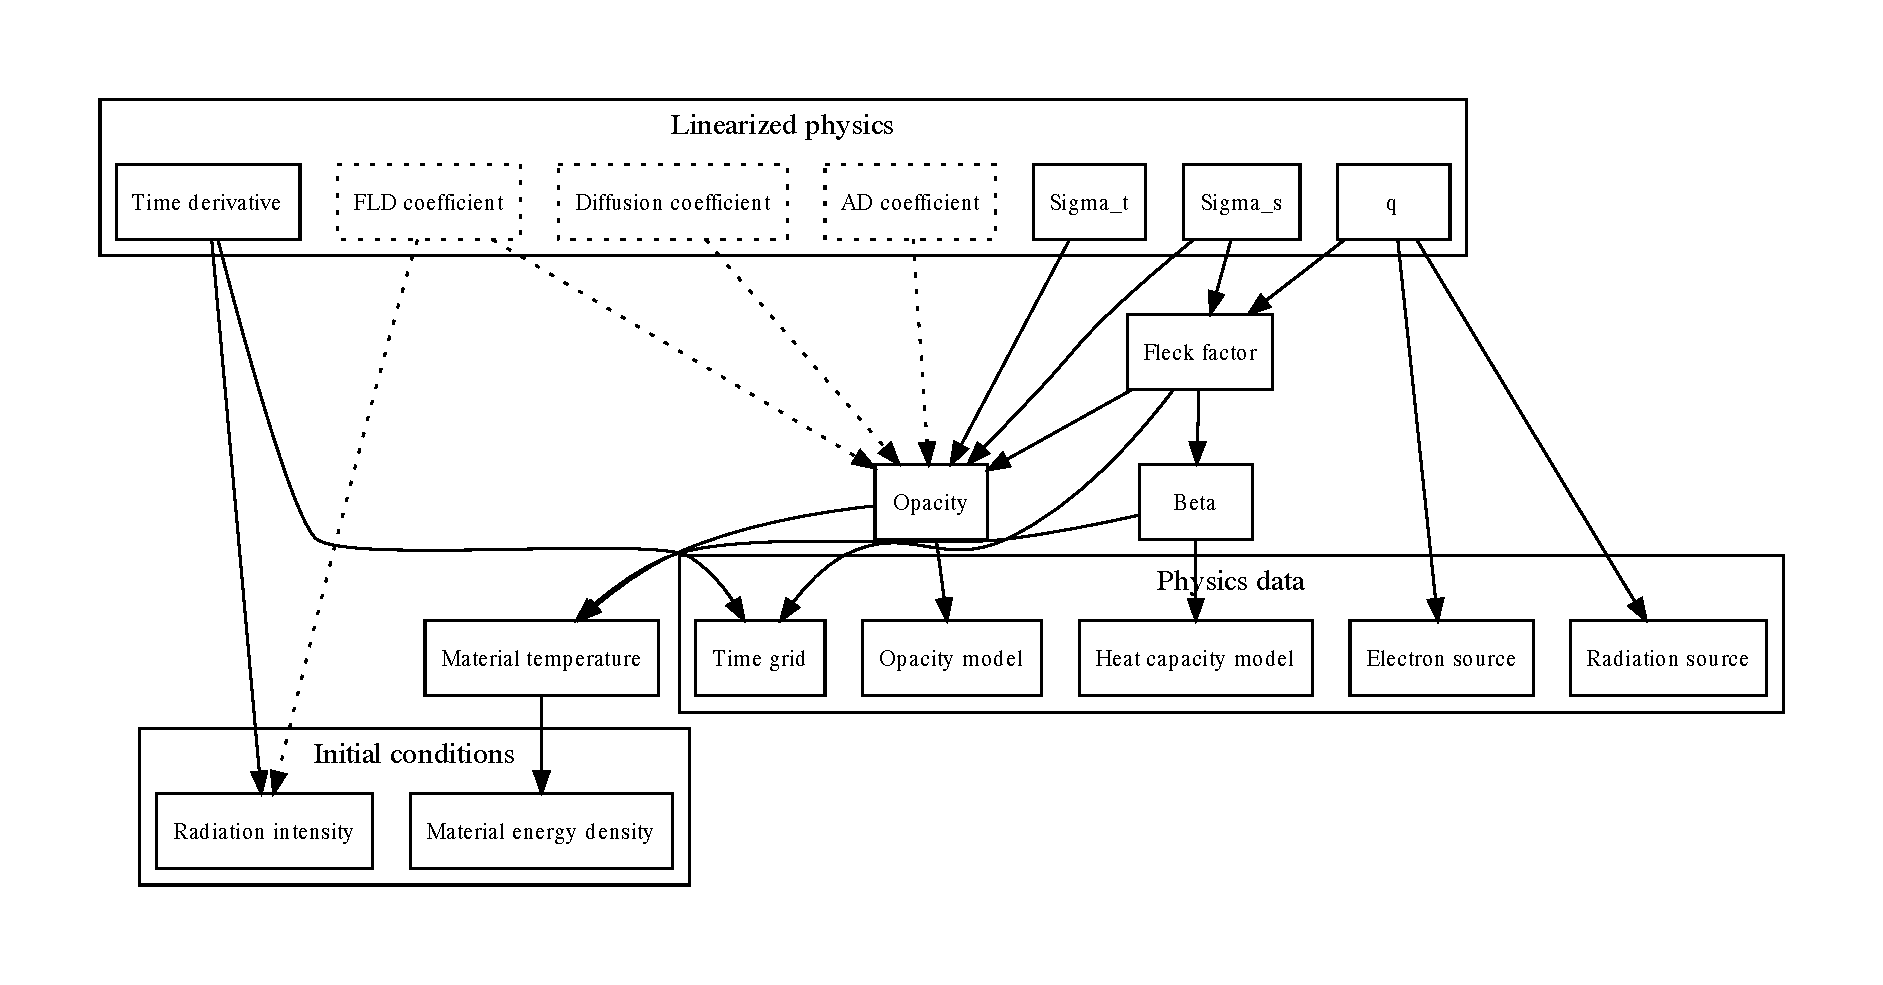
\includegraphics[width=8in]{semi-implicit}
  \caption{Dependency graph of quantities in the semi-implicit discretization.}
  \label{fig:semiImplicitFlowchart}
\end{sidewaysfigure}

